\section{Arduino kode med én sensor}
Den indledende løsning blev først implementeret på en Arduino Uno mikrocontroller hvorefter konceptet blev testet og verificeret. Koden er derfor i sin indledende fase også skrevet i Arduino.

\begin{figure}[h!]
  \centering
  \includegraphics[width=1.0\textwidth]{figures/followLine2.png}
  \caption{FollowLine() funktion.}
  \label{follow_line_kode}
\end{figure}

På figur \ref{follow_line_kode} ses funktionen follow\_Line(). Koden fungerer sålades at når sensoren registrerer den hvide omkringliggende farve drejes der til højre og når den sorte linje registreres drejes der til venstre. Robotten kører derved kun på kanten af linjen. 

Ved brug af én sensor har gruppen valgt at anvende et referencepunkt til sammenligning med målinger. Dette referencepunkt kaldet mean\_value i koden, er gennemsnittet for den sorte streg og den hvide baggrund. Herefter hvis målingen er under gennemsnittet, drejes til den ene siden, og er den over drejes til den anden side.\fxnote{find ud af om det ikke er for tæt på det der står ved flowchartet}
\newpage



\section{Test og delkonklussion}
Testen er udført ved hjælp af en legomindstorm bane i oval form.
Ud fra det introducerde linetrack system blev konceptet testet ved brug af én sensor på den opstillede bane. 
\newline
Robotten fuglte den sorte streg 

Ud fra denne test kan det konkluderes at softwaren virker i henhold til den indledende problemløsning. Robotten er i stand til at følge kanten af linjen ved hjælp af de forskellige overfladefarveværdier som sensoren registrerede gennem testen. 
\newline

\begin{figure}[h!]
  \centering
  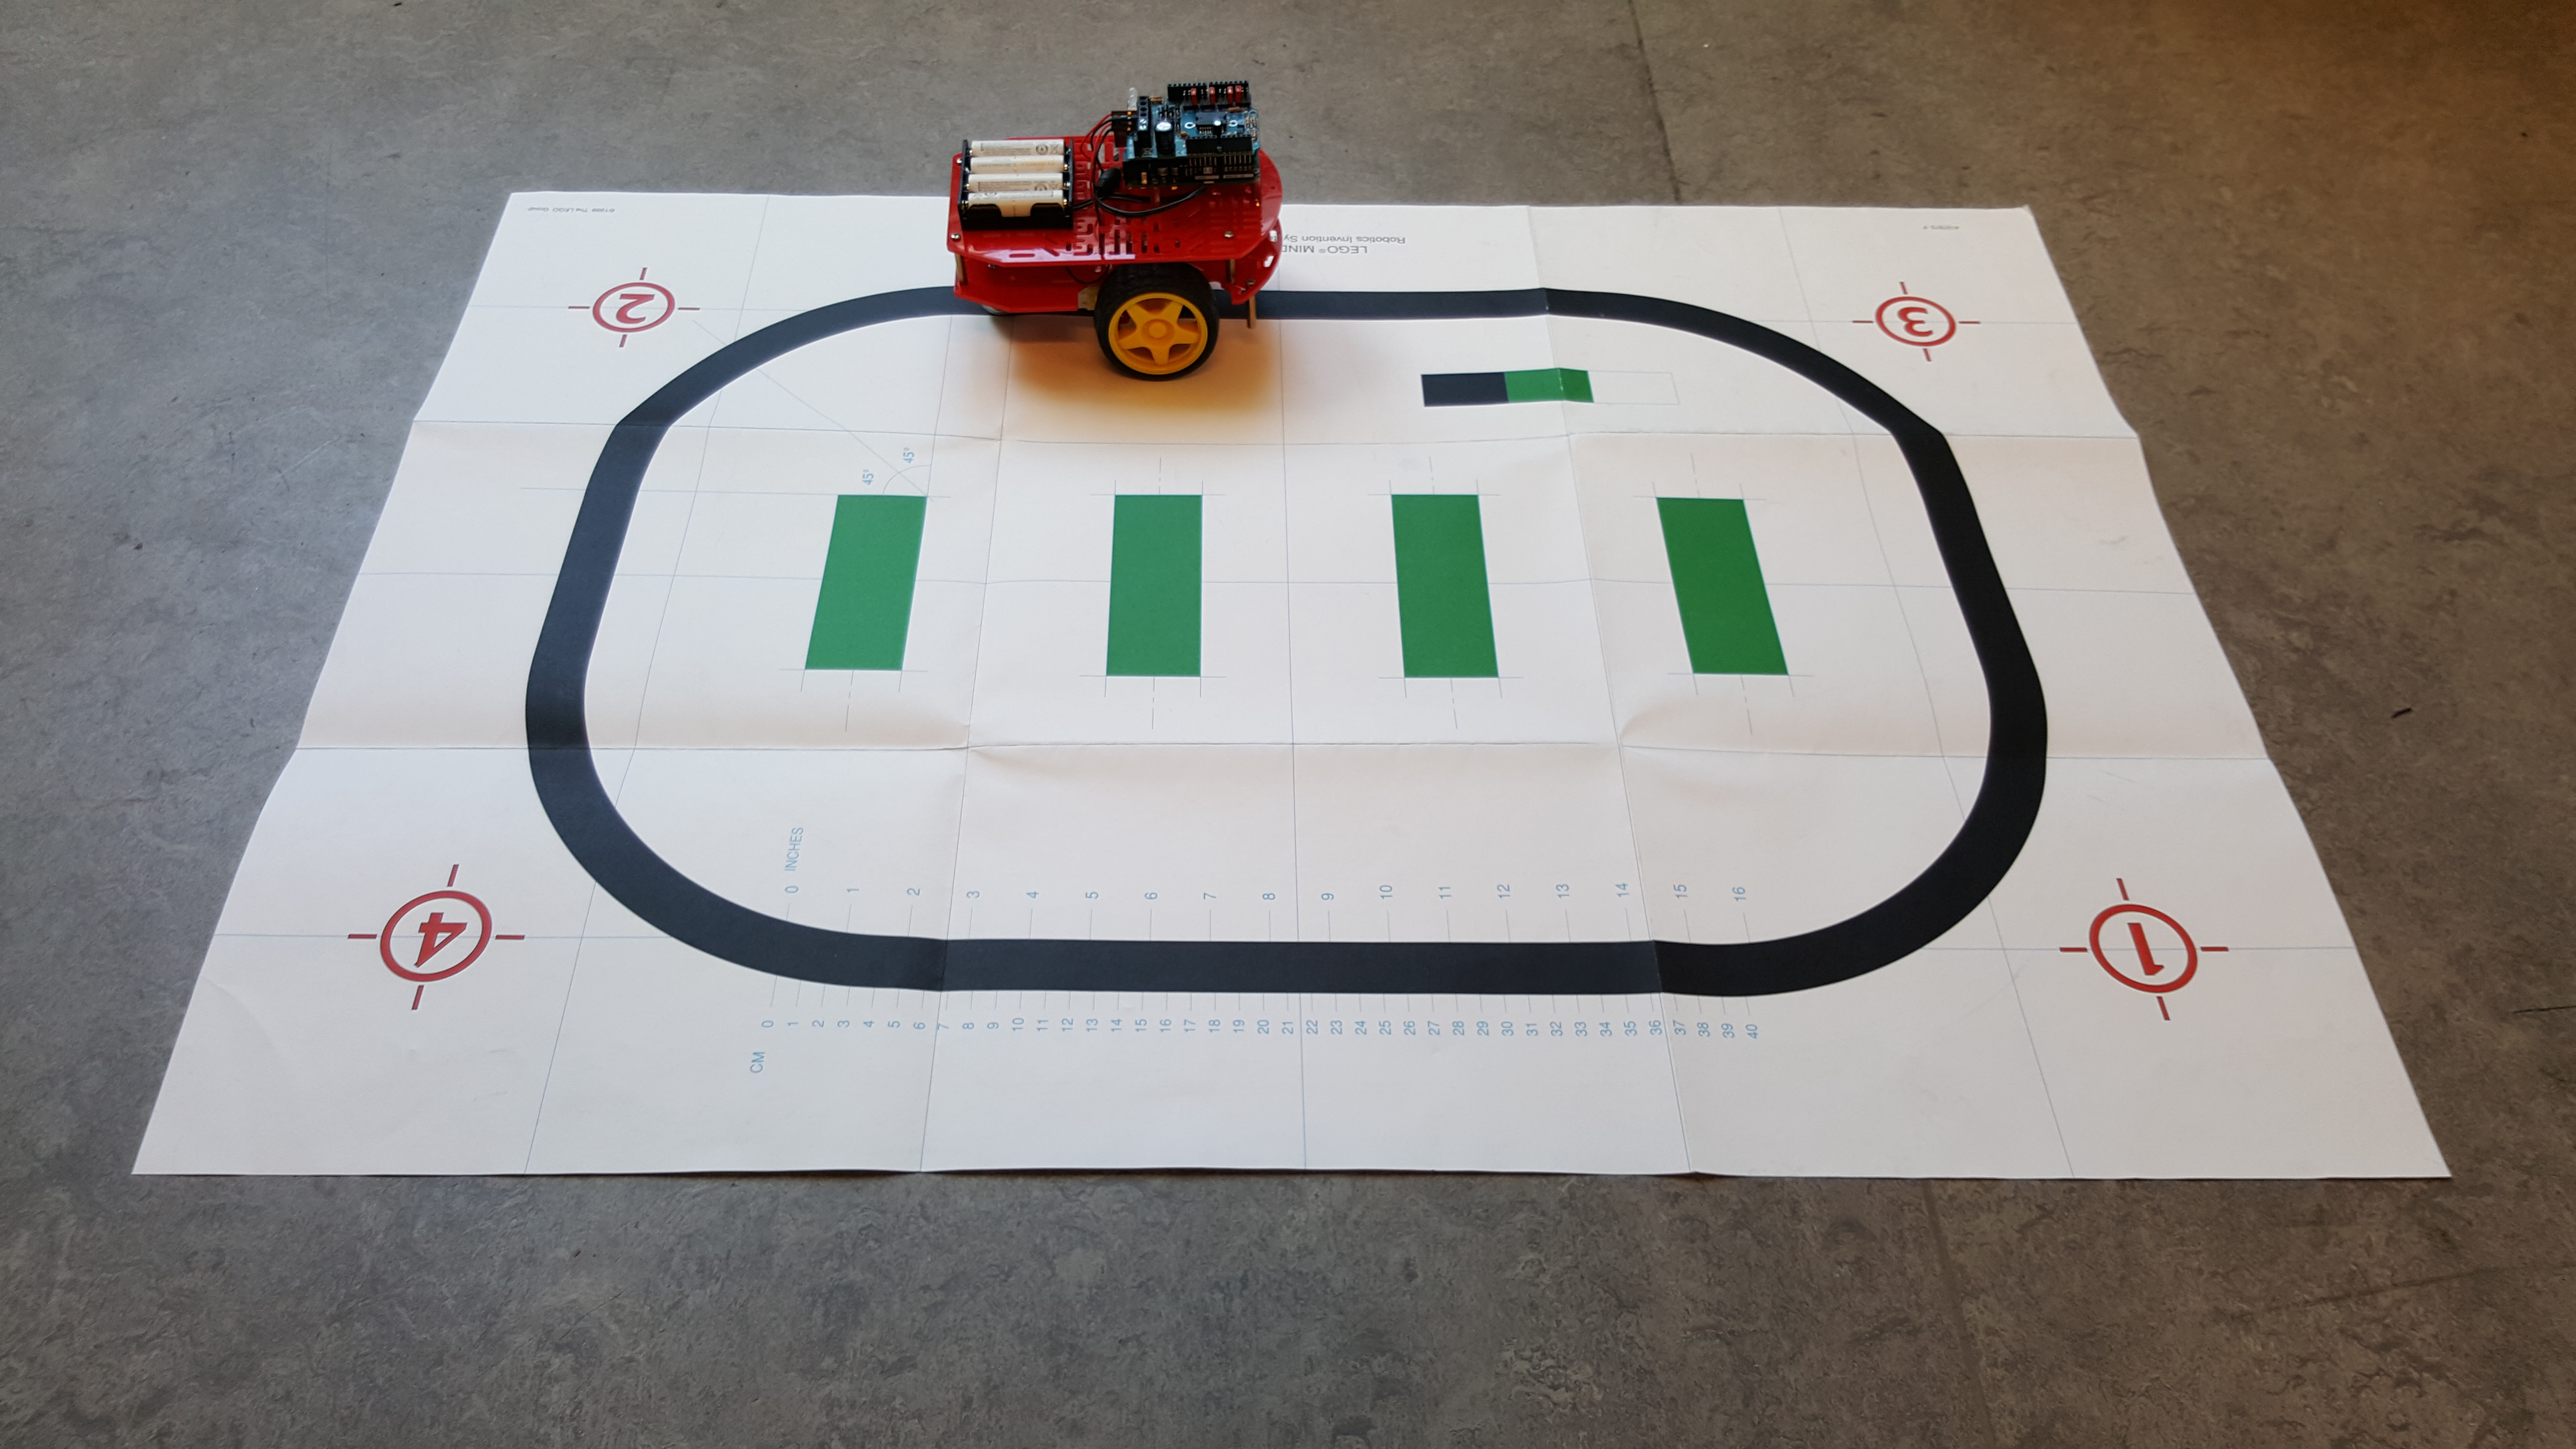
\includegraphics[width=0.6\textwidth]{figures/testMedEnSensor.png}
  \caption{Den inledende software løsning til linetrackinging med 1 sensor i et superloop.}
  \label{indledende_test}
\end{figure}
\newpage



 

